
\setcounter{chapter}{6}

\chapter{Embodiment in humanoid robots}
\label{c:embodiment}


In this third part we will apply the lexicon formation models from the
previous three chapters with to real-world situated interactions of
autonomous robots. We will discuss mechanisms and representations for
conceptualization that allow to link words to the visual perceptions
of the robots and we will analyze what impact the additional
challenges and complexities coming from embodiment and
conceptualization have on the performance of these models. But in
order to do that, we will first dedicate one chapter to the perceptual
and social skills that we endowed the robots with for engaging in
grounded language games\footnote{Some parts of of the first two
  sections of this chapter are taken from \cite*{loetzsch12grounding}
  and additionally appeared in shorter form in
  \cite*{spranger12perceptual}.}.

\begin{figure}[p]
  \begin{tabular}{lr}
    \multicolumn{2}{l}{\includegraphics[width=1\textwidth]{figures/photo-qrio-1}} \\
    & \\
    & \\
    \includegraphics[width=0.48\textwidth]{figures/photo-qrio-3} &
    \includegraphics[width=0.48\textwidth]{figures/photo-qrio-2} \\
    & \\
  \end{tabular}
  \caption{The Sony humanoid robot.}
  \label{f:photo-qrio}
\end{figure}


We used two ``Sony humanoid robots'' (\citealp{fujita03autonomous},
see Figure \ref{f:photo-qrio}) for all of our robotic
experiments. They are about 60 cm high, weigh approximately 7 kg and
have 38 degrees of freedom (4 in the head, 2 in the body, 5$\times$2
in the arms, 6$\times$2 in the legs and 5$\times$2 in the
fingers). The main sensors are three CCD cameras in the head, of which
we used here one. The camera delivers up to 30 images per second, has
an opening angle of about 120$^\circ$ and a resolution of
176$\times$144 pixels. It uses the $YCrCb$ color space ($Y$: luma or
brightness, $Cr$: chroma red and $Cb$: chroma blue) with 8 bits per
channel. Furthermore, the robots have three accelerometers and gyro
sensors in the trunk and one accelerometer in each foot. The feet are
equipped with force feedback sensors to detect ground contact. The
batteries have enough capacity for about an hour of autonomous
operation.

We endowed the robots with a vision system for recognizing and
tracking objects in their environment. This system is explained in
Section \ref{s:vision-system} and Section
\ref{s:joint-attention-and-social-skills} introduces a set of social
skills for engaging in language games that were programmed into the
robots. Finally, in Section \ref{s:doing-experiments-with-robots} we
describe the overall experimental setup, i.e. how more high-level
cognitive processess for conceptualization and language interact with
the sensori-motor capabilities of the robots, and we characterize some
properties of the sensory experiences that the robots construct.



\section{Visual object recognition and tracking}
\label{s:vision-system}

\begin{figure}[t]
  \includegraphics[width=1\textwidth]{figures/vision-system-stages-overview}
  \caption{Image processing steps for three subsequent points in
    time. A: Source images provided by the camera of the robot. B:
    Foreground/ background classification and motion detection (blue
    rectangles). Foreground regions are then associated to existing
    object models or become seeds for new object representations. C/D:
    The changing histogram of the green-red channel for object
    $o_{716}$ is used to track $o_{716}$ in space and time and thus to
    create a persistent model of the object. E: Knowing the offset and
    orientation of the camera relative to the body, the robots are
    able to estimate the position and size of objects in the
    world. Black arrows denote the positions of the two robots
    perceiving the scene.}
\label{f:vision-system-overview}
\end{figure}

The environment of the robots consists of a variety of physical
objects such as toys, cones, barrels and cuboids (see Figure
\ref{f:object-sets}, page \pageref{f:object-sets}) that are initially
unknown to the robots. Objects are frequently added to the scene and
removed again. In addition, objects are moved within a scene and their
appearance may alter. For example the red block in Figure
\ref{f:vision-system-overview}A is standing up in the beginning and is
then put down, changing the perception of the object from being high
and thin to low and broad. In addition, perceiving objects is made
difficult by partial occlusions and other interfering factors such as
human experimenters manipulating the objects in front of the robots.

A prerequisite for building the internal cognitive structures needed
for communicating about objects is that the robots have mechanisms for
constructing perceptual representations of the objects in their
immediate surroundings from the raw sensations streaming from the
robots' sensors. Constructing such representations involves three
sub-systems: First, low-level vision routines process raw camera
images to yield basic \emph{percepts} -- connected regions that differ
from the background of the environment. Figure
\ref{f:vision-system-overview}B gives an example and the mechanisms
involved are explained in Section \ref{s:detecting-foreground-regions}
below. Second, these foreground regions are tracked in subsequent
camera images despite changing positions and appearances of the
objects. In order to do so, the vision system needs to establish a
correspondence between an internal \emph{object model} and the image
regions that refer to the same physical object, a process known in
robotics as \emph{anchoring}
\citep{coradeschi03anchoring,loutfy05maintaining}. For example as
illustrated in Figure \ref{f:vision-system-overview}D, the changing
raw sensations for the red block in Figure
\ref{f:vision-system-overview}A are continously connected to the same
\emph{anchor} $o_{716}$. We used \emph{Kalman Filters} for maintaining
such persistent object models (Section \ref{s:object-models}). Third,
when needed in communicative interactions, the vision system encodes a
set of visual properties about each object model. In this particular
setup these properties are the object's position in a robot egocentric
reference system, an estimated width and height and color information,
as shown in Figure \ref{f:vision-system-overview}E. This process is
discussed further in Section \ref{s:computing-object-features}.


\subsection{Detecting foreground regions in images}
\label{s:detecting-foreground-regions}

The robots do not know in advance what kind of objects to expect in
their environment. Thus, the assumption is made that everything that
was not in the environment before is considered to be a potential
object. The system, therefore, gathers statistical information about 
the environment's background in a calibration phase 
and image regions that sufficiently differ from the background are 
treated as candidates for object models. 
For generating a statistical model of the scene
background, the robots observe the experiment space without objects
for some time (see Figure \ref{f:photo-calibration-phase}) and
perceive a series of calibration images such as in Figure
\ref{f:object-perception}A. For all three color channels $c \in
\{Y,Cr,Cb\}$ the mean $\mu_{c,\vec{p}}$ and variance
$\sigma_{c,\vec{p}}^2$ of the image intensities at every image pixel
$\vec{p}$ are computed over all calibration images. After the
calibration phase the robots are presented with objects, resulting in
raw camera images such as in Figure \ref{f:object-perception}B. The
generated background statistics are used to classify all image pixels
as being foreground or background. A pixel is considered foreground
when the difference between the image intensity $i_c(\vec{p})$ and the
mean of that pixel is bigger than the pixel's standard deviation
($\mid i_c(\vec{p}) - \mu_{c,\vec{p}}\mid > \sigma_{c,\vec{p}}$) for
one of the color channels $c \in \{Y,Cr,Cb\}$. As a result, a binary
image as shown in Figure \ref{f:object-perception}C is generated with
all foreground pixels having the value of $1$ and all others $0$.

\begin{figure}[t]
  \includegraphics[width=0.65\textwidth]{figures/vision-system-photo-calibration-phase}
  \caption{Calibration phase of the vision system. Both robots are
    shown an empty environment for some extended period of time,
    allowing them to observe the statistical characteristics of the
    scene background.}
  \label{f:photo-calibration-phase}
\end{figure}

\begin{figure}[t]
  \centerline{\footnotesize\sffamily 
    \renewcommand{\arraystretch}{2.0}
    \begin{tabular}{@{}l@{}p{0.025\textwidth}@{}l@{}p{0.025\textwidth}@{}l@{}p{0.025\textwidth}@{}l@{}p{0.025\textwidth}@{}l@{}}
      A & & B & & C & & D \\
      \includegraphics[width=0.23\textwidth]{figures/vision-system-object-perception-1} & &
      \includegraphics[width=0.23\textwidth]{figures/vision-system-object-perception-2} & &
      \includegraphics[width=0.23\textwidth]{figures/vision-system-object-perception-3} & &
      \includegraphics[width=0.23\textwidth]{figures/vision-system-object-perception-4} \\
      E & & F & & G & & H \\
      \includegraphics[width=0.23\textwidth]{figures/vision-system-object-perception-5} & &
      \includegraphics[width=0.23\textwidth]{figures/vision-system-object-perception-6} & &
      \includegraphics[width=0.23\textwidth]{figures/vision-system-object-perception-7} & &
      \includegraphics[width=0.23\textwidth]{figures/vision-system-object-perception-8} \\
    \end{tabular}}
  \caption{From foreground regions to object models. A: A raw camera
    image taken during the calibration phase. B: A camera image of a
    scene containing objects. C: The result of foreground/ background
    classification. White pixels are foreground, green pixels were not
    classified. D: The noise-reduced classification image. E: The
    segmented foreground regions drawn in their average color and with
    bounding boxes. Note that the partially overlapping blue and green
    blocks in the right bottom of the original image are segmented
    into the same foreground region. F: Classification of foreground
    pixels using existing color models. Pixels are drawn in the
    average color of the most similar object model. G: Bounding boxes
    and average colors of the segmented classification image. Note
    that the use of previous color models helped to generate separate
    percepts for the blue and green blocks at the right bottom of the
    image. H: Kalman filtered object models. The state bounding boxes
    are drawn in the average color of the model. I: Computation of
    position and size in a robot-egocentric reference system. The
    width and height of objects is indicated by the width and height
    of the triangles.}
  \label{f:object-perception}
\end{figure}

This binary image is further noise-reduced using standard image
operators (dilatation, erosion, see for example
\citealp{parker96algorithms,soille02morphological}) as illustrated in
Figure \ref{f:object-perception}D. First, noise is removed through
applying a $3\times 3$ erosion operator. Second, the change in size of
regions caused by the erosion operator is compensated by applying a
$3\times 3$ dilation operator. Then a segmentation algorithm scans the
filtered image and computes for all connected foreground pixels a
surrounding polygon, the bounding box, and color histograms of the
pixels contained in the region (for each color channel, from the
original image). Color histograms $M^c$ represent frequencies of image
intensities on the color channel $c$, computed either over complete
images or parts of them in the case of foreground regions. The whole
range of intensities is divided into $m$ bins $k~\in~\{1,\dots,m\}$ of
equal size. The number of pixels that have intensities falling into
each bin $M^c(k)$ is counted using a function $h(i_{c}(\vec{p}))$ that
assigns the intensity $i_c$ of a pixel $\vec{p}$ to a bin
$k$. Normalized histograms $\hat{M}^c(k)$ are computed from such
histograms by dividing each frequency $M^c(k)$ by the number of pixels
sampled, resulting in a representation where the sum of all
$\hat{M}^c(k)$ for $k~\in~\{1,\dots,m\}$ is equal to $1$, allowing to
interpret $\hat{M}(h(i_c(\vec{p})))$ as the probability of an image
intensity to occur in an image (or a sub-region). Figure
\ref{f:object-perception}E shows the estimated bounding boxes and
average colors extracted from the regions.



Objects frequently occlude each other, due to particular spatial
placement, but also when moved around in the scene.  For example the
green cube is partly overlapping the blue cuboid in the right bottom
of Figure \ref{f:object-perception}B and thus the segmentation
algorithm creates only one foreground region for both
objects. Provided that there is an established object model (see next
Section \ref{s:object-models}) for at least one of the objects, it is
possible to further divide such regions. Each pixel in a foreground
region is assigned to the most similar color model of previously
perceived objects as shown in Figure \ref{f:object-perception}F. Given
the normalized color histograms $M_I^c$ of all pixels in the current
image $I$ and $M_1^c,\dots,M_n^c$ of the $n$ previously established
object models, the likelihood $p_j$ of a pixel $\vec{p}$ in a
foreground region to belong to a color model $j$ can be calculated:

$$p_{j}(\vec{p})=M^Y_{j}(h(i_Y(\vec{p}))) \cdot M_{j}^{Cr}(h(i_{Cr}(\vec{p}))) \cdot M_{j}^{Cb}(h(i_{Cb}
(\vec{p})))$$

\noindent Based on this probability, each pixel is either classified
to belong to the model $j$ with the highest likelihood
$\operatorname{class}({\vec{p}})=\arg\max_{j=1..n}(p_{i}(\vec{p}))$
or, when the highest $p_{j}$ is smaller than a threshold $t$ or when
no previous model exists, to a ``no model'' class. Classified pixels
are again segmented into connected regions. As shown in Figures
\ref{f:object-perception}G and \ref{f:object-perception}H, the
initially connected foreground region for the blue and green objects
in the right bottom of the image could be divided into separate
regions due to the use of previous color models.


The resulting subdivided foreground regions are called
\emph{percepts}.  They represent the result of the low-level image
processing mechanisms acting separately on each image without
incorporating past knowledge (except for the color information of
previous objects). A percept $P$ is defined as $P:=\langle
x_P,y_P,w_P,h_P,M_P^Y,M_P^{Cr},M_P^{Cb},n_P\rangle$ with $x_P,y_P$
describing the center of the percepts bounding rectangle in image
coordinates, $w_P$ and $h_P$ the width and height of the bounding
rectangle in pixels, $M_P^Y$, $M_P^{Cr}$ and $M_P^{Cb}$ the normalized
histograms for the three color channels and $n_P$ the number of pixels
contained in the region.\\

\noindent In order to improve the tracking algorithm described in the next
Section, we also implemented a component for identifying regions in
the image where motion has occured. Image intensities
$i_{c,t}(\vec{p})$ at time $t$ are compared to those of images taken
at time $t-1$. A pixel $\vec{p}$ is classified as subject of motion
when the difference is bigger than the standard deviation
$\sigma_{c,\vec{p}}$ of this pixel's intensities calculated during the
calibration phase ($\mid i_{c,t}(\vec{p}) - i_{c,t-1}(\vec{p})\mid >
\sigma_{c,\vec{p}}$) for one of the color channels $c
\in\{Y,Cr,Cb\}$. The resulting classification image is noise-reduced
and segmented into regions of motion as shown in Figure
\ref{f:vision-system-overview}B. This information is used to loosen
the parameters for the association of percepts to object models.  If
there is motion in a particular region of the image, then object
models are allowed to move and change color more drastically than if
there is no motion.



\subsection{Maintaining persistent object models}
\label{s:object-models}

For maintaining a set of stable and persistent models of the objects
in their environment, the robots have to associate the percepts
extracted from each raw image to existing object models. Furthermore,
they have to create new models when new objects enter the scene and
eventually delete some models when objects disappear. This task is
difficult because objects can move and the detection of regions
through foreground/background separation is noisy and
unreliable. Extracted properties such as size or position may highly
vary from image to image and it can happen that objects are only
detected in some of the images streaming from the camera.


The internal object model $O_t$ of an object at time step $t$
(whenever a new camera image is processed) is defined as $O_t:=\langle
id_O,s_{O,t},\Sigma_{O,t},M^Y_{O,t},M^{Cr}_{O,t},M^{Cb}_{O,t}\rangle$,
with $id_{O}$ being an unique id serving as an anchor for the object,
$s_{O,t}$ a state vector capturing spatial properties, $\Sigma_{O,t}$
the $8 \times 8$ state covariance matrix and $M_{O,t}^Y$,
$M_{O,t}^{Cr}$ and $M_{O,t}^{Cb}$ normalized color histograms. A state
vector $s$ is defined as $s_{O,t}:=\begin{pmatrix} x_{O,t} & y_{O,t} &
  w_{O,t} & h_{O,t} & \dot{x}_{O,t} & \dot{y}_{O,t} & \dot{w}_{O,t} &
  \dot{h}_{O,t}\end{pmatrix}^T$, with $x_{O,t},y_{O,t}$ describing the
center of the object in the image, $w_{O,t}$ and $h_{O,t}$ the
object's width and the height in pixels and $\dot{x}_{O,t}$,
$\dot{y}_{O,t}$, $\dot{w}_{O,t}$ and $\dot{h}_{O,t}$ the change
variables (speed of change in position and size).

We use Kalman Filters \citep{kalman60new} to model the spatial
component $s_{O,t}$ of object models. In every time step $t$ all Kalman
Filter states $s_{O,t-1}$ and $\Sigma_{O,t-1}$ of the last time step $t-1$
are used to \emph{predict} a new a priori state $\overline{s}_{O,t}$ and a
state covariance matrix $\overline{\Sigma}_{O,t}$ given the $8\times8$
state transition matrix $A$ and the process noise covariance matrix
$Q$:
\begin{eqnarray*}
\overline{s}_{O,t}&:=&As_{O,t-1} \\ 
\overline{\Sigma}_{O,t}&: =& A \Sigma_{O,t-1} A^T+Q
\end{eqnarray*}
We found it sufficient to use a constant state transition matrix $A$,
which predicts every dimension via its change variable
and a constant noise covariance matrix $Q=1^{-5}\cdot I_8$.

Next attempts are made to associate percepts to existing models.
Since the position, dimension and color of objects change over time,
no a priori known invariant properties of objects allow to decide
which percept belongs to which model. Instead, a similarity score
$\hat{s}$ based on position and color is used. The score reflects a
set of assumptions and heuristics, which are based on intuitive
notions of how objects behave, so that experimenters can change the
scene, without having to adjust to particular properties of the vision
system.  First it is assumed that an object can not randomly jump in
the image or disappear at one point in space and appear at
another. Consequently, a spatial similarity $\hat{s}_{euclid}$ can be
defined using the Euclidean distance between the center of a percept
$P$ and the predicted position $\overline{x}_{O,t},\overline{y}_{O,t}$
of a model $O$

$$
\hat{s}_{euclid}(P,O):=1 - \frac{\sqrt{(x_P-\overline{x}_{O,t})^2+(y_P-\overline{y}_{O,t})^2}}{l}
$$

\noindent with $l$ being the length of the image diagonal in
pixels. The result of $\hat{s}_{euclid}$ is $1$ when the two points
are identical and $0$ when they are in opposite corners of the image.
Since objects are assumed to move in a predictable fashion, a
threshold $t_{space}$ restricts the radius around a model in which
percepts are associated -- the spatial association score
$\hat{s}_{space}$ equals to $\hat{s}_{euclid}$ when it is bigger than
$t_{space}$ and $0$ otherwise. Second, it is assumed that objects do
not change their color in a random fashion. An object's color
histogram that has a very high value in a certain bin will not have a
zero value in that bin in the next image. Percepts and object models
can thus be compared using a color similarity $\hat{s}_{color}$. It is
based on the Bhattacharyya coefficient $BC$
\citep{bhattacharyya43measure,aherne98bhattacharyya} that is used as a
similarity measure between two normalized histograms $M$ and $M'$:

$$BC(M,M'):=\sum_{k=1}^{m}\sqrt{M(k) \cdot M'(k)}$$

\noindent Using the color histograms $M_P^c$ of a percept $P$ and the
histograms $M_{O,t-1}^c$ of a previous model $O$, a similarity measure
combining all three color channels is defined as:

$$
\hat{s}_{Bhatt}(P,O) := \prod_{c \in \{Y,Cr,Cb\}} BC(M^c_P,M^c_{O,t-1})
$$

\noindent The association score $\hat{s}_{color}(P,O)$ then yields the
result from the above measure when it is bigger than a threshold
$t_{color}$ or $0$ otherwise. In order to allow more rapid changes in
space and color when objects move, the two association thresholds
$t_{space}$ and $t_{color}$ are loosened when motion has been detected
within the area spawned by a state.

The overall similarity score between a particular percept and an
existing object model is then defined as:

$$\hat{s}(P,O)= \hat{s}_{space}(P,O) \cdot \hat{s}_{color}(P,O)$$

\noindent Each percept is associated with the internal state that has
the highest association non-zero score $\hat{s}$ with respect to that
percept. If no such state exists (when either the spatial or color
similarity is below the threshold), then the percept is stored in a
list of unassociated percepts.

  
\begin{figure}[t]
  \parbox{0.486\textwidth}{%
    \includegraphics[width=0.23\textwidth]{figures/vision-system-object-modeling-1}%
    \hspace{0.025\textwidth}%
    \includegraphics[width=0.23\textwidth]{figures/vision-system-object-modeling-2}}
  \caption{Kalman filtered object models. The state bounding boxes are
    drawn in the average color of the model and the state covariance
    is visualized with the thin cross in the center of each model.}
  \label{f:object-modeling}
\end{figure}

The Kalman Filter states are \emph{updated} given the associated
percepts, which are beforehand combined into a single percept.
Percepts are combined by computing a bounding polygon and a histogram
representing the color frequency in the combined region.  Using the
predicted a priori state vector $\overline{s}_{O,t}$ and state
covariance $\overline{\Sigma}_{O,t}$ as well as the spatial components
$p$ of the combined percept $p:=\begin{pmatrix}x_P&y_P
  &w_P&h_P\end{pmatrix}^T$, the a posteriori state $s_{t}$ and the a
posteriori state covariance matrix $\Sigma_{O,t}$ are computed

\begin{eqnarray*}
  K_{O,t}&=&\overline{\Sigma}_{O,t} H^T H\overline{\Sigma}_{O,t}H^T+R\\
  s_{O,t}&=&\overline{s}_{O,t}+K_{O,t}(p-H\overline{s}_{O,t})\\
  \Sigma_{O,t}&=&(I-K_{O,t}H)\overline{\Sigma}_{t}
\end{eqnarray*}

\noindent with $R$ as the constant $4\times4$ measurement covariance
matrix (with $R=1^{-1}\cdot I_4$) and $H$ a constant $8\times4$ matrix
relating the measurement space and the state space (with $h_{i,j}=1$
for all $i=j$ and $0$ for all others). In principle $H$ and $R$ are
allowed to change over time, but the above estimates resulted in
sufficient tracking performance.  Additionally, the color histograms
of a state $S$ are updated using

$$M^c_{O,t}(k):=(1-\alpha) M^c_{O,t-1}(k)+\alpha M^c_{P}(k)$$

\noindent for all color channels $c\in\{Y,Cr,Cb\}$, all histogram bins
$k\in\{1,\dots,m\}$ and with $\alpha \in [0,1]$ being the influence
of the combined percept.

New object models are created from unassociated percepts. All
unassociated percepts lying in the same foreground region are combined
and used as a seed for a new model which is assigned a new
unique ID.  In order to avoid creating models from percepts generated
for body parts of the experimenter, new models are only created when
no motion was detected. Models that have not been associated
with percepts for some time are deleted. This mainly happens when
objects disappear from the scene and consequently no percepts are
associated with them. As a result of the modeling process, Figure
\ref{f:object-modeling} shows the object models at the time when the
percepts in Figure \ref{f:object-perception} were generated.


\subsection{Computing object features}
\label{s:computing-object-features}

From each object model, a set of features such as color, position and
size are extracted. These feature vectors are called \emph{sensory
  experiences} and are used by the agents to construct the different
conceptual entities needed for engaging in the different kind of
language games introduced in this thesis.

\begin{figure}[t]
  \includegraphics[width=0.75\textwidth]{figures/vision-system-coordinate-systems}
  \caption{Computation of object positions on the ground plane, size
    estimation and the involved coordinate systems. Note that all
    systems except the image coordinate system are three
    dimensional. }
  \label{f:vision-system-coordinate-systems}
\end{figure}


The two robots can perceive the environment from arbitrary angles,
which makes the position and size of objects in the camera image bad
features for communicating about objects. For example the width of an
object in the image depends on how far the object is away from the
robot and is thus not at all shared by the robots. In order to be
independent from how objects are projected onto camera images, spatial
features are computed in an egocentric coordinate system relative to
the robot. However, without the use of stereo vision or a priori known
object sizes, positions can not be determined solely from camera
images. But given the reasonable assumption that objects are located
on the ground, they can be calculated by geometrically projecting
image pixels onto the ground plane using the offset and rotation of
the camera relative to the robot as shown in Figure
\ref{f:vision-system-coordinate-systems}. The egocentric robot
coordinate system originates between the two feet of the robot, the
$z$ axis is perpendicular to the ground and the $x$ axis runs along
the sagittal and the $y$ axis along the coronal plane. First, a
virtual image projection plane orthogonal to the optical axis of the
camera is used to relate image pixels in the two-dimensional image
coordinate system to the three-dimensional camera coordinate system
(which has its origin in the optical center of the camera, with the
$x$ axis running along the optical axis and the $y$ and $z$ an axis
being parallel to the virtual image plane). Given the camera
resolution height and width $r_{w}$ and $r_{h}$ (in pixels) as well as
the horizontal and vertical camera opening angle $\phi_{v}$ and
$\phi_{h}$, the $x_i$ and $y_i$ coordinates of an image pixel can be
transformed into a vector $\vec{v}_c$ in the camera coordinate system

$$
\vec{v}_{c}= \begin{pmatrix}1\\
  -\frac{x_i}{r_{h}} \cdot \tan\frac{\phi_{h}}{2}\\
  \frac{y_i}{r_{v}} \cdot \tan\frac{\phi_{v}}{2}\\
\end{pmatrix}
$$

\noindent that ``points'' to the pixel on the virtual projection
plane. Given the orientation of the camera relative to the robot
represented by the $3\times3$ rotation matrix $R_{c}$, a vector
$\vec{v}_c$ can be rotated into a vector $\vec{v}_t$ in the camera
translated coordinate system (which originates in the center of the
camera, with the axes being parallel to the robot coordinate system)
with $\vec{v}_{t}=R_{c} \cdot \vec{v}_{c}$. Furthermore, given the
offset from the origin of the robot coordinate system to the center of
the camera $\vec{t}_{c}$, the position of a pixel projected onto the
ground plane $\vec{v}_r$ in the egocentric robot coordinate system can
be computed by intersecting the ray $\vec{v}_{t}$ with the ground
plane using simple geometric triangulation: The equation

$$
\vec{v}_r= a \cdot \vec{v}_t + \vec{t}_c
$$

\noindent with the unknown scalar $a$ has exactly one solution for
$x_r$ and $y_r$ when the pixel designated by $\vec{v}_t$ lies below
the horizon.  The operating system of the Sony humanoid readily
provides estimates for $R_{c}$ and $\vec{t}_{c}$ that are computed
from joint sensor values.

Using these transformations, the position features {\tt x} and {\tt y}
(in mm) are extracted from an object model by projecting the pixel at
the center of the lower edge of the object's bounding box onto the
ground plane. For estimating a {\tt width} feature, the lower left and
right corner of a the bounding box are transformed into positions
relative to the robot and the distance between them is calculated. For
the computation of {\tt height}, the ray of the pixel on the middle of
the upper bounding box edge is intersected with a virtual plane
perpendicular to the ground and through the position of the object as
shown in Figure \ref{f:vision-system-coordinate-systems}.  The
extraction of color features from object models is also
straightforward. The feature {\tt luminance} is computed as the mean
of an internal state's color histogram $M_t^{Y}$, {\tt green-red} as
the mean of $M_t^{Cr}$ and {\tt yellow-blue} from
$M_t^{Cb}$. % Similarily, the {\tt stdev-luminance}, {\tt
%   stdev-green-red} and {\tt stdev-yellow-blue} features are the
% standard deviations of the color histograms $M_t^c$ and express how
% uniform the image pixels perceived for an object are.

\begin{figure}[t]
  \parbox{0.75\columnwidth}{%
    \vspace{-3mm}\hspace{3mm}%
    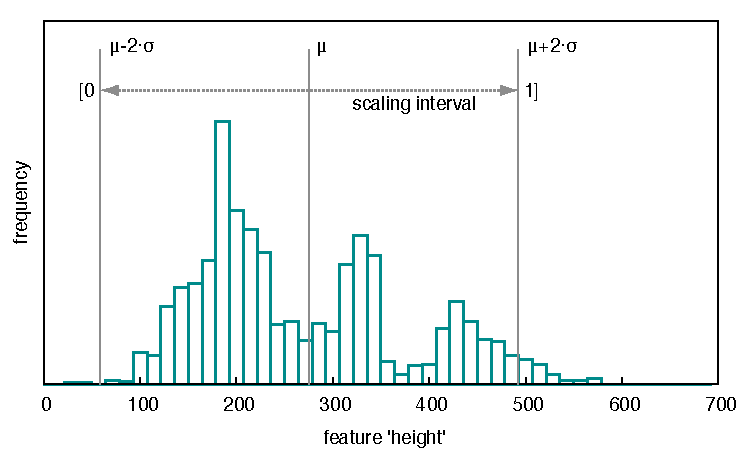
\includegraphics[width=0.75\columnwidth]{figures/vision-system-scaling}}
  \caption{Scaling of feature values. The distribution of the 'height'
    feature sampled over all objects of the geometric objects data set
    (see Section \ref{s:recording-data-sets} on page
    \pageref{s:recording-data-sets}) is used to define an interval
    $\mathsf{[\mu-2\sigma,\mu+2\sigma]}$ for scaling feature values
    into the interval $\mathsf{[0,1]}$.}
  \label{f:vision-system-scaling}
\end{figure}

\begin{figure}[t]
  \parbox{\textwidth}{\fontsize{2.25mm}{2.5mm}\sffamily 
  \includegraphics[width=1\textwidth]{figures/vision-system-example-scene}
  \vspace{1mm}
  
  \renewcommand{\arraystretch}{1.5}
  \newcommand{\sub}[1]{\raisebox{-2pt}{\tiny#1}}
  \addtolength{\tabcolsep}{-2.4pt}
  \definecolor{dark}{rgb}{0.5,0.2,0}     
  \hskip0.5mm\begin{tabular*}{\textwidth}{@{}p{17.5mm}|rl|rl|rl||rll|rll|rll@{}}
    & \multicolumn{6}{c||}{experience robot A} & \multicolumn{9}{c}{experience robot B} \\
    feature & 
    \multicolumn{2}{c}{o\sub{708}} & 
    \multicolumn{2}{c}{o\sub{716}} &
    \multicolumn{2}{c||}{o\sub{722}} & 
    \multicolumn{3}{c}{o\sub{712}} & 
    \multicolumn{3}{c}{o\sub{718}} & 
    \multicolumn{3}{c}{o\sub{725}} \\
    \hline
    x & 464 & 0.43 & 821 & 0.69 & 686 & 0.59
    & 607 & 0.53 & \itshape\textcolor{dark}{0.11}
    & 925 & 0.76 & \itshape\textcolor{dark}{0.08}
    & 432 & 0.40 & \itshape\textcolor{dark}{0.19} \\
    y & 151 & 0.61 & 17 & 0.51 & 453 & 0.82
    & -301 & 0.28 & \itshape\textcolor{dark}{0.33}
    & 137 & 0.60 & \itshape\textcolor{dark}{0.09}
    & 115 & 0.58 & \itshape\textcolor{dark}{0.25} \\
    width & 47 & 0.31 & 150 & 1.00 & 46 & 0.30
    & 62 & 0.46 & \itshape\textcolor{dark}{0.15}
    & 196 & 1.00 & \itshape\textcolor{dark}{0.00}
    & 45 & 0.29 & \itshape\textcolor{dark}{0.01} \\
    height & 116 & 0.35 & 138 & 0.42 & 67 & 0.19
    & 109 & 0.33 & \itshape\textcolor{dark}{0.02}
    & 186 & 0.58 & \itshape\textcolor{dark}{0.16}
    & 135 & 0.41 & \itshape\textcolor{dark}{0.22} \\
    luminance & 126 & 0.76 & 72 & 0.30 & 81 & 0.37
    & 130 & 0.79 & \itshape\textcolor{dark}{0.03}
    & 57 & 0.17 & \itshape\textcolor{dark}{0.13}
    & 85 & 0.41 & \itshape\textcolor{dark}{0.03} \\
%     stdev-luminance & 41 & 0.71 & 23 & 0.39 & 22 & 0.36
%     & 39 & 0.69 & \itshape\textcolor{dark}{0.03}
%     & 15 & 0.24 & \itshape\textcolor{dark}{0.15}
%     & 20 & 0.33 & \itshape\textcolor{dark}{0.04} \\
%     min-luminance & 35 & 0.40 & 40 & 0.48 & 29 & 0.31
%     & 26 & 0.26 & \itshape\textcolor{dark}{0.14}
%     & 39 & 0.46 & \itshape\textcolor{dark}{0.02}
%     & 27 & 0.27 & \itshape\textcolor{dark}{0.03} \\
%     max-luminance & 199 & 0.79 & 185 & 0.69 & 126 & 0.30
%     & 198 & 0.78 & \itshape\textcolor{dark}{0.01}
%     & 139 & 0.39 & \itshape\textcolor{dark}{0.30}
%     & 126 & 0.30 & \itshape\textcolor{dark}{0.00} \\
    green-red & 206 & 0.81 & 187 & 0.72 & 101 & 0.29
    & 206 & 0.81 & \itshape\textcolor{dark}{0.00}
    & 196 & 0.76 & \itshape\textcolor{dark}{0.04}
    & 98 & 0.28 & \itshape\textcolor{dark}{0.01} \\
%     stdev-green-red & 17 & 0.71 & 22 & 0.93 & 8 & 0.29
%     & 17 & 0.71 & \itshape\textcolor{dark}{0.00}
%     & 9 & 0.35 & \itshape\textcolor{dark}{0.58}
%     & 8 & 0.30 & \itshape\textcolor{dark}{0.01} \\
%     min-green-red & 149 & 0.76 & 129 & 0.64 & 80 & 0.34
%     & 139 & 0.70 & \itshape\textcolor{dark}{0.06}
%     & 151 & 0.77 & \itshape\textcolor{dark}{0.13}
%     & 76 & 0.31 & \itshape\textcolor{dark}{0.02} \\
%     max-green-red & 233 & 0.79 & 253 & 0.89 & 126 & 0.27
%     & 232 & 0.79 & \itshape\textcolor{dark}{0.00}
%     & 252 & 0.89 & \itshape\textcolor{dark}{0.00}
%     & 123 & 0.26 & \itshape\textcolor{dark}{0.01} \\
    yellow-blue & 119 & 0.53 & 110 & 0.47 & 99 & 0.38
    & 121 & 0.55 & \itshape\textcolor{dark}{0.02}
    & 123 & 0.57 & \itshape\textcolor{dark}{0.10}
    & 97 & 0.37 & \itshape\textcolor{dark}{0.02} \\
%     stdev-yellow-blue & 4 & 0.32 & 22 & 1.00 & 9 & 0.53
%     & 4 & 0.31 & \itshape\textcolor{dark}{0.00}
%     & 4 & 0.29 & \itshape\textcolor{dark}{0.71}
%     & 9 & 0.53 & \itshape\textcolor{dark}{0.00} \\
%     min-yellow-blue & 100 & 0.56 & 39 & 0.12 & 72 & 0.36
%     & 102 & 0.58 & \itshape\textcolor{dark}{0.01}
%     & 95 & 0.53 & \itshape\textcolor{dark}{0.41}
%     & 72 & 0.36 & \itshape\textcolor{dark}{0.00} \\
%     max-yellow-blue & 132 & 0.45 & 133 & 0.46 & 124 & 0.38
%     & 132 & 0.45 & \itshape\textcolor{dark}{0.00}
%     & 140 & 0.52 & \itshape\textcolor{dark}{0.06}
%     & 126 & 0.40 & \itshape\textcolor{dark}{0.02} \\
    \hline
  \end{tabular*}
  \vspace{3mm}
  
}


% (defparameter *world* (make-instance 'physical-robot-world :data-sets '("qrio-1")))
%
% (defparameter *objects* (list (third (entities (get-world-model *world* "scene-3378523360" 'a)))
% 			    (fifth (entities (get-world-model *world* "scene-3378523360" 'a)))
% 			    (fourth (entities (get-world-model *world* "scene-3378523360" 'a)))
% 			    (third (entities (get-world-model *world* "scene-3378523360" 'b)))
% 			    (fifth (entities (get-world-model *world* "scene-3378523360" 'b)))
% 			    (fourth (entities (get-world-model *world* "scene-3378523360" 'b)))))
%
% (loop for i from 0 to 16
%    do (format t "~%      ~(~a~)" (fname (nth i (features (first *objects*)))))
%      (loop for object in (subseq *objects*  0 3)
% 	do (format t " & ~d & ~,2f" (round (value (fvalue (nth i (features object))))) (value (fvalue (nth (+ i 17) (features object))))))
%      (loop for object in (subseq *objects*  3 6)
% 	for j from 3
% 	do (format t "~%      & ~d & ~,2f & \\itshape\\textcolor{dark}{~,2f}" (round (value (fvalue (nth i (features object))))) 
% 		   (value (fvalue (nth (+ i 17) (features object))))
% 		   (abs (- (value (fvalue (nth (+ i 17) (features object)))) (value (fvalue (nth (+ i 17) (features (nth (- j 3) *objects*)))))))))
%      (format t " \\\\"))

%%% Local Variables: 
%%% mode: latex
%%% TeX-master: "../phdbook"
%%% End: 

  \caption{Snapshots of the sensory experiences of both robots at the
    end of the image sequence in Figure
    \ref{f:vision-system-overview}. Top: The camera images at that
    point in time are overlaid with the object anchors maintained by
    the tracking system. Left of them, the positions of objects and
    other robots in the egocentric reference system of each robot are
    shown. Each object is drawn as a circle in its average color, with
    the radius representing the object's width. The positions of the
    two robots (see Section \ref{s:extimating-robot-position} below)
    are indicated using black arrows. Bottom: The actual feature
    values are shown in each first column and feature values scaled to
    the interval $[0,1]$ in each second column.  On the right side of
    the table, the third columns give for each scaled feature the
    difference between the perception of robot A and B.}
  \label{f:vision-system-example-scene}
\end{figure}

The values of the {\tt x} and {\tt y} features are ususally in the
range of meters, {\tt width} and {\tt height} can range from a few
centimeters up to half a meter and values on color channels are within
the interval $[0,255]$. In order to be able to handle all features
independently from the dimensions of their domains, feature values are
scaled to be within the interval $[0,1]$ using the statistical
distributions of feature values as illustrated in Figure
\ref{f:vision-system-scaling} In theory the robots could gradually
build up such distributions by seeing many different objects over the
course of time, in practice the distributions are sampled from objects
of recorded data sets (see Section \ref{s:recording-data-sets}). Given
the mean $\mu$ and standard deviation $\sigma$ of the distribution of
a feature over a (large) number of objects, a scaled value is computed
%$$\overline{v}:=\min(1,\max(0,\frac{v-\mu}{4\cdot\sigma}+\frac{1}{2}))$$
by mapping values in the interval $\mathsf{[\mu-2\sigma,\mu+2\sigma]}$
onto $\mathsf{[0,1]}$ and clipping all others. Figure
\ref{f:vision-system-example-scene} gives an example of the sensory
experiences of the two robots. For each object, both the unscaled and
scaled feature values are given.


\subsection{Visual perception in humans and robots}

The psychological and neurobiological literature on vision contains a
lot of evidence for correlates of these three sub-systems in the human
brain. First, there are dedicated neural assemblies along the visual
stream from the retina to the primary visual cortex that detect basic
visual features on a number of separable dimensions such as color,
orientation, spatial frequency, brightness and direction of movement.
These \emph{early vision} processes operate independently from
attention to objects and features ``are registered early,
automatically, and in parallel across the visual field ''
\citep[p. 98]{treisman80feature-integration}. From there on, two
separate visual pathways (also known as the ``what'' and ``where''
systems) are responsible for identifying objects and encoding
properties about them (see \citealp{mishkin83object} for an early
review): A dorsal stream (the ``where'' system) connecting the primary
visual cortex and the posterior parietal cortex is responsible for the
primitive individuation of visual objects, mainly based on spatial
features. ``Infants divide perceptual arrays into units that move as
connected wholes, that move separately from one another, and that tend
to maintain their size and shape over motion''
(\citealp{spelke90principles}, p. 29). These ``units'' can be
understood as ``pointers'' to sensory data about physical objects that
enable the brain for example to count or grasp objects without having
to encode their properties. They can be compared to the \emph{anchors}
mentioned above and are subject of a large number of studies:
\cite{marr82vision} calls them \emph{place tokens},
\cite{pylyshyn01visual,pylyshyn89role} \emph{visual indexes},
\cite{ballard97deictic} \emph{deictic codes} and
\cite{hurford03neural} discusses them from an artificial intelligence
and linguistics perspective as \emph{deictic variables}. In a second
ventral stream (the ``what'' system) running to the infero-temporal
cortex, properties of objects are \emph{encoded} and temporarily stored in
the \emph{working memory} \citep{baddeley86working-memory} for the use
in other cognitive processes. What these properties are depends on
top-down attentional processes -- for example different aspects of objects
have to be encoded when a subject is asked to count the number of
``big objects'' vs. the number of ``chairs''.


In addition to findings from neuroscience, there is also a variety of
previous work in robotics to rely on. The most widely known setups for
grounding symbolic representations in visual data for the purpose of
communication is probably the Talking Heads experiment
(\citealp{steels98origins}, see \citealp{belpaeme98construction} for
details of the vision system). Static scenes consisting of geometric
shapes on a blackboard are perceived by robotic pan-tilt cameras and
the vision system is able to extract features such as color, size and
position from these shapes. \cite{siskind95grounding} describes a
computer program for creating hierarchical symbolic representations
for simple motion events from simulated video input and in
\citep{siskind01grounding} from real video sequences (see also
\citealp{baillie00action,steels03shared,dominey05learning} for very
similar systems and \citealp{chella00understanding,chella03anchoring}
for a comparable framework inspired by the \emph{conceptual spaces} of
\citealp{gardenfors00conceptual-spaces}).

Furthermore, there is a vast literature on object detection and
tracking algorithms for other purposes than symbol grounding (see
\citealp*{yilmaz06object-tracking} for an extensive review). And the
vision system introduced here does not reinvent the wheel but makes
use of well-established techniques such as color histograms and Kalman
filters. It differs, however, from many other approaches in the notion
of what is considered to be an object. The types of objects that are
expected to occur in the world are often explicitly represented in the
vision system, for example by using pre-specified color ranges for
identifying different object classes in images
(e.g. \citealp{perez02color-based}), by matching (sometimes learnt)
object templates with images (e.g. \citealp{hager98efficient}) or by
engineering dedicated algorithms tailored for recognizing specific
classes of objects (e.g. \citealp*{juengel04real-time}). 

In contrast, our robots have no preconceptions of what to expect in
their environment and thus can detect and track any type of object,
using only two assumptions: First, everything appearing in the
environment that sufficiently distinguishes itself from the background
and that was not there before is considered to be an object. Second,
objects have to be on the ground for being able to make reliable
position and size estimates. Furthermore, what makes the approach
presented here quite special is the tight integration of visual
perception with other cognitive mechanisms such as social behavior
(see below), conceptualization and language (as discussed in the
next chapters).


\section{Joint attention \& mechanisms for social learning in robots}
\label{s:joint-attention-and-social-skills}

Robots learning a language are not only grounded in the physical world
through their sensorimotor apparatus but also socially grounded in
interactions with others. In addition to perceptual capabilities for
detecting and tracking objects in their environment they need a set of
social skills for engaging in communicative interactions with each
other. This includes mechanisms for joint attention and pointing as
well as behavioral scripts for structured conversations. Joint
attentional scenes \citep{tomasello95jointattention} ``are social
interactions in which the child and the adult are jointly attending to
some third thing, and to one another's attention to that third thing,
for some reasonably extended length of time''
\citep[p. 97]{tomasello99cultural}. Establishing joint attention means
in our robotic experiments that two robots taking part in a language
game must (1) share a physical environment, (2) attend to a set of
objects in their surrounding, (3) track whether the respective other
robot is able to attend to the same set of objects and (4) be able to
manipulate attention by pointing to distal objects and perceiving
these pointing gestures (see Figure \ref{f:qrio-pointing}).

\begin{figure}[t]
  \parbox{0.7\textwidth}{ \includegraphics[width=0.7\textwidth]{figures/qrio-pointing-photo-of-scene}
    
    \vspace{0.03\textwidth}\includegraphics[width=0.335\textwidth]{figures/qrio-pointing-camera-image-b}\hspace{0.03\textwidth}\includegraphics[width=0.335\textwidth]{figures/qrio-pointing-camera-image-a}
  }
  \caption{Demonstration of a Sony humanoid robot drawing the
    attention of the other robot to an object in the shared
    environment by pointing at it. The images at the right show the
    scene as seen through the camera of the pointer (top) and the
    robot observing the pointing (bottom). However, please note that
    the robots are not able to detect pointing gestures using their
    built-in cameras. Instead, they directly transmit $x,y$
    coordinates of the object pointed at.}
  \label{f:qrio-pointing}
\end{figure}

\subsection{Social robotics}

How social mechanisms can be implemented in robots is a research area
in its own. Scientist in this field are mainly interested in how
social skills can improve communication and collaboration between
humans and robots \citep{breazeal02designing}. Additionally, by trying
to endow robots with social behaviors that appear ``natural'' to human
observers, they want to understand what social cues humans are
responding to. For reviews, refer to \cite*{dautenhahn02from} who
developed taxonomies for different degrees of robots' embodiment and
``social embeddedness'', \cite*{fong03survey} who give a general
survey of socially interactive robots, and \cite{vinciarelli09social}
who review the field of ``social signal processing'', i.e. the
detection of social cues in human behavior.  For an overview of skills
that are prerequisites for joint attention and the state of the art in
robotic experiments trying to implement these skills, refer to
\cite{kaplan06challenges}. Some examples of work relevant for the
experiments in this paper are listed below.

\cite{scassellati99imitation} endowed the ``Cog'' robot
\citep{brooks99cog} with capabilities for finding human faces,
extracting the location of the eye within the face, and determining if
the eye is looking at the robot for maintaining eye contact (or mutual
gaze). \cite*{marjanovic99self-taught} showed how the same robot could
learn to control his arm for pointing at distal objects in the
surrounding space, guided by the camera of the robot.  Gaze
recognition was investigated among many others by
\cite{kozima01robot}. They demonstrated how the ``Infanoid'' robot is
able to track gaze direction in human faces and use this information
to identify objects that humans are looking at. Joint attention is
established by alternatingly looking at distal objects and the
faces. \cite{nagai03constructive} modeled the transitions between
different developmental stages that infants are going through in the
process of learning to engage in joint attentional scenes, resulting
in the robot being able to determine which object a human caregiver is
looking at.


For recognizing pointing gestures performed by humans,
\cite*{kortenkamp96recognizing} developed a robot that can detect and
track the 3D positions of arm and shoulder joints of humans in dynamic
scenes, without requiring the humans to wear special markers. By
searching along the vector defined by the detected arm joints, the
robot can determine which object the experimenter was pointing
at. Similarly, \cite{martin09estimation} used pointing gestures to
instruct a mobile robot where to navigate to. \cite*{colombo03visual}
used multiple cameras for tracking humans pointing at areas on walls
in a room.  \cite{nickel07visual} equipped a robot with stereo cameras
and use color and disparity information and Hidden Markov Models to
track both the direction of gaze and the position where a human is
pointing at.  \cite{haasch05multi-modal} apply the ability to
recognize pointing gestures for teaching words for objects in a
domestic environment and \cite*{imai03physical} showed how the robot
"Robovie" could combine mechanisms for establishing mutual gaze and
pointing at objects to draw the attention of humans to a poster in the
environment of the robot. Finally, \cite{hafner05learning}
demonstrated how recognition of pointing gestures could be learned in
Aibo robots. One robot performs a hard-wired pointing gesture and the
other one has to detect whether it was to the left or to the right.

Additionally there is considerable research into implementing and
learning the necessary behaviors for engaging in structured
conversations.  \cite{breazeal03sociable} investigated turn taking
with the Kismet robot, focussing on the factors regulating the
exchange of speaking turns so that the communication seems natural to
human interlocutors.  \cite{cassell99turntaking} discussed how
nonverbal gestures and gaze can support turn taking behaviors in
multimodal dialogs with the embodied conversational agent (ECA)
``Gandalf'', trying to replicate findings from psychologic data. A bit
more on the theoretical side, \cite{iizuka03adaptive} followed a
Dynamic Systems approach for understanding processes of cognition and
action \citep{thelen94dynamic} to understand turn-taking in wheeled
mobile robots in terms of the underlying dynamics of recurrent neural
networks. Recent work on communication with ECAs is reviewed by
\cite{kroeger09model} for the co-ordination of communicative bodily
actions across different modalities and by \cite{kopp10social} for the
alignment of communicative behaviors between interlocutors.



\subsection{Implementing language games in robots}
\label{s:scaffolding-social-skills}

Language games are coordinated by behavioral scripts (see Section
\ref{s:language-game}, page \pageref{s:language-game}). Every agent in
the population knows the language game script and individually reacts
to changes in the environment and actions of the other robot. For
example the speaker triggers the action of pointing to the intended
topic when the hearer signals that he did not understand the
utterance. The scripts are implemented in the form of finite-state
machines: actions are performed depending on the current state in the
game flow, the perception of the environment and the history of the
interaction (see also \citealp*{loetzsch06xabsl}).

Joint attention is monitored by an external computer program, that has
access to the world models of both interacting robots.  This system
initiates the interaction between two agents as soon as both agents
observe the same set of objects.  It is the task of the human
experimenter to find spatial setups in which joint attention is
possible, the program only monitors whether robots are seeing the same
set of objects. But in the literature there are also other proposals
for establishing joint attention in embodied language game
experiments. For example \cite{steels97grounding} programmed
sophisticated signaling protocols into LEGO robots. A robot that
decides to become a speaker emits an infrared signal and the other
robot then aligns its position so that it faces the speaker. The
robots ``point'' to objects by orienting themselves toward them. In
the Talking Heads experiment \citep{steels98origins}, the speaker
directly controls the view direction of the hearer's camera in order
to make sure that their cameras perceive the same objects on the
whiteboard. An agent points to an object by letting the other agent's
camera zoom in on it. In contrast, establishing joint attention in
social language learning scenarios between humans and robots is
usually easier because the human experimenter (as a well-trained
social being) is good at monitoring the attention of the robot and can
for example (as in \citealp{dominey05learning}) point to an object by
moving it.


For constructing a naming system robots need non-linguistic means of
conveying information, such as pointing to an object or conveying
notions of success, failure and agreement in communication.  For
demonstration purposes robots were equipped with behaviors for
pointing at objects (see Figure \ref{f:qrio-pointing}). We used motion
teaching for creating a set of 18 pointing motions for different areas
in front of the robot. Depending on the $x,y$ coordinate of the object
to point at, the pointing routines selects and performs one of these
pre-taught motions. 

Nevertheless, in the communicative interactions underlying the
experiments presented here, robots use a different mechanism in order
to avoid further difficulties stemming from uncertainties in pointing
(see \citealp{steels98stochasticity} for a disscussion of the impact
of such uncertainties on the performance in language games). When a
robot wants to point to an object in the environment, he directly
transmits the $x_o,y_o$ coordinates of the intended object $o$ to the
interlocutor.  Since robots model object positions in their own
(egocentric) coordinate systems, additional steps have to be taken to
interpret these coordinates.  Most importantly the robot has to know
the position $x_r,y_r$ and orientation $\theta_r$ of the robot that is
pointing $r$ (see next Section \ref{s:extimating-robot-position} for
details on how robots estimate these values).  With this information
robots transform the coordinates into their own coordinate system:

$$
\vec{v}=\begin{pmatrix} \cos \theta_r & -\sin \theta_r \\ \sin
  \theta_r & \cos \theta_r \end{pmatrix} \begin{pmatrix} x_o \\
  y_o\end{pmatrix} + \begin{pmatrix} x_r \\ y_r\end{pmatrix}
$$

\noindent The robot interpreting the pointing is determining the
intended object by choosing the object in his world model that is
closest to $\vec{v}$. Furthermore, although we implemented gestures
for giving non-linguistic communicative feedback (nodding the head for
success and shaking for failure) and we used the built-in speech
synthesizer of the Sony humanoid robots for producing utterances,
feedback signals whose meaning is shared and utterances are directly
passed between
interlocutors.\\

\noindent The mechanisms presented in this Section provide simple solutions to
required capacities for social language learning that are not meant to
be in themselves proposals as to how these skills could be
implemented. Nevertheless, we claim that the realism of this study
does not suffer from this simplicity: humans rely on extremely
powerful mechanisms for perceiving and sharing intentions within
interactive situations \citep{tomasello05understanding} and similarly
our solutions provide us with the technical prerequisites for letting
our robots learn from communicative interactions.



\subsection{Robot pose estimation}
\label{s:extimating-robot-position}

A requirement for the pointing mechanisms described above is a quite
precise estimate of the position and orientation of the other
robot. For that, robots localize themselves with respect to landmark
objects in the environment and transmit their position with respect to
these landmarks to the other robot. This way both agents establish
mutual knowledge about their position. We use carton boxes enhanced
with visual markers (see Figure \ref{f:artoolkit}) as landmark
objects.  The unique, black and white, barcode-like, 2D-patterns
attached to carton boxes are tracked using the ARToolKitPlus library
\citep{wagner07artoolkitplus}, which is an improved version of
ARToolKit \citep{kato99marker,kato00virtual}, especially adapted for
mobile devices.

\begin{figure}[t]
  \begin{tabular}{lr}
    \multicolumn{2}{l}{
      \includegraphics[width=0.6\columnwidth]{figures/artoolkit-0}\vspace{4mm}} \\
    \includegraphics[width=0.28\columnwidth]{figures/artoolkit-1} & 
    \includegraphics[width=0.28\columnwidth]{figures/artoolkit-2}\vspace{4mm}\\
    \includegraphics[width=0.28\columnwidth]{figures/artoolkit-3} & 
    \includegraphics[width=0.28\columnwidth]{figures/artoolkit-4}\\
  \end{tabular}
  \caption{Using objects enhanced with visual markers for estimating
    the position and orientation of the other robot. Top: Example of a
    carton box that is enhanced with 2D patterns. Center left: A
    carton box with markers as seen through the camera of a Sony
    humanoid robot. Center right: Binary image generated from the
    original image.  Bottom left: The marker as detected by the
    ARToolKit tracking system. Bottom right: Both robots send the
    position and orientation of the carton box (blue) to each other
    and are thus able to deduce the position and orientation of the
    respective other robot. }
  \label{f:artoolkit}
\end{figure}

From each camera image, a histogram of the pixel luminance is
computed. This histogram is then used to derive a threshold for
creating a binary image as shown in the top right of Fig.
\ref{f:artoolkit}. The binary image is passed to the tracking library,
which searches it for marker patterns and determines the four vertices
of the polygon surrounding the marker in the image (see bottom left of
Fig. \ref{f:artoolkit}). Provided with the camera resolution width
and height (in pixels), the width and height camera opening angle (in
deg) and the widths of the markers used on the carton boxes (in mm),
the tracking library is able to make an orientation and position
estimate from the edges of the detected patterns, which is then
iteratively enhanced by matrix fitting. As a result, the system
returns for each detected marker pattern a unique ID and a matrix
describing the position and orientation of the marker relative to the
camera of the robot (for details of the pose estimation algorithm
see \citealt*{kato99marker}).

To transform the camera relative marker position and orientation into
robot egocentric coordinates, they are transformed using the offset
and orientation of the camera relative to the ground point of the
robot (see Section \ref{s:computing-object-features}).  Finally, for
each marker attached to a carton box, the offset and orientation
relative to the center of the box, which is a priori known, is used to
determine the position and orientation of the box in egocentric
coordinates. To filter out noise and recognition errors, the resulting
box poses are averaged over the last $n$ images. Also, when two
markers of the same box are detected in the same image, their
resulting box poses are averaged.  The output of the landmark modeling
system is a list of objects consisting of an ID (an ID of the box, not
to confuse with the ID of the marker patterns) and a pose
$\vec{b}:=\begin{pmatrix}x_b & y_b & \theta_b\end{pmatrix}$ of the
carton box in robot egocentric coordinates.


In order to determine the position $x_r,y_r$ and orientation
$\theta_r$ of the respective other robot, the robots use the carton
boxes as global landmarks (see bottom right of Fig.
\ref{f:artoolkit}). About five times per second they exchange the
poses of the boxes they have seen over a wireless network
connection. Given that both robots see the same box (all robots use
the same box IDs for the same visual markers), they can compute the
pose of the other robot from the box pose $\vec{b}$ as perceived by
the robot (in egocentric coordinates) and the $\vec{b}'$ as sent by
the other robot (in the coordinate system of the other robot):

$$
\begin{pmatrix} x_r \\ y_r \\ \theta_r \end{pmatrix} 
:= 
\begin{pmatrix} 
x_b - \cos(\theta_b - \theta_b') \cdot x_b' + \sin(\theta_b - \theta_b') \cdot y_b'  \\
y_b - \cos(\theta_b - \theta_b') \cdot x_b' + \sin(\theta_b - \theta_b') \cdot x_b'  \\
\theta_b - \theta_b'
\end{pmatrix}
$$

\noindent When both robots see multiple boxes the results of the above
transformation are averaged.



\section{Experimental setup}
\label{s:doing-experiments-with-robots}

Integrating all the mechanisms for visual perception and behavior
control into a complete setup for doing language game experiments is a
challenging but also interesting task in its own (see
\citealp{thorisson07integrated} for a discussion of ``integrated
A.I. systems''). It requires computational infrastructure for
connecting single components into a fast and robust system and proper
modularization is needed in order to be able to develop and test
algorithms and behaviors separately. Furthermore, for understanding
the complex dynamics of the experimental setup and for detecting
problems or errors, it is crucial to have visualizations for each
single step in the information processing. Finally, in order to be
able to do repeatable experiments and for testing components without
actually working on a real robot, mechanisms for recording and
replaying each intermediate result of the system are a necessity.

\subsection{Computational infrastructure}

\begin{figure}[t]
  \parbox{\textwidth}{
  \includegraphics[width=0.48\textwidth]{figures/computer-infrastructure-1}%
  \hspace{0.04\textwidth}%
  \includegraphics[width=0.48\textwidth]{figures/computer-infrastructure-2}%
  \vspace{0.04\textwidth}
  
  \includegraphics[width=1\textwidth]{figures/computer-infrastructure-network}%
  \vspace{3mm}}
\caption{Computational infrastructure. Top left: five computers were
  involved in conducting the experiments. Top right: real-time
  visualizations of the vision system. Bottom: schematic view of the
  connections between the different subsystems. The robots communicate
  with gateway computers over a wireless network and the computers are
  connected trough an Ethernet network.}
  \label{f:computational-infrastructure}
\end{figure}

The components of the experimental setup are distributed over five
different machines (see Figure \ref{f:computational-infrastructure}),
which is mainly due to the fact that the software involved was written
for different operating systems. The vision system runs in real-time
on an external Microsoft Windows PC (one for each robot). It was
developed on the basis of the 2004 version of the framework used by
the GermanTeam \citep{roefer04germanteam} for participating in the
RoboCup \citep{kitano97robocup} Sony Four Legged League. The
GermanTeam's framework is written in C++ and consists of an
architecture for modularizing tasks, mechanisms for exchanging data
across processes and platforms and a set of powerful debugging
mechanisms \citep{roefer03architecture}.  Besides that, the framework
contains the program \emph{RobotControl}, an application for
visualizing nearly every aspect of the vision system (see top right
image of Figure \ref{f:computational-infrastructure}) and for
debugging and testing components. RobotControl is also used for
recording data to external hard drives and it translates requests from
the language game system (see below) into representations that are
used by the robotic software.

The software running on the Sony humanoid robots was provided by the
members of the Sony Intelligent Systems Research Labs and we used it
without modification. Running on top of the Aperios operating system,
Open-R \citep{fujita97open,ishida01motion} is responsible for
collecting data from sensors and controlling actuators. There are
high-level behavioral primitives for issuing walking commands, gazing
at points in space, performing arm movements, speech output and
more. In the background the system constantly monitors the body
stability and tries to balance walking and other motions, as described
in \citep{nagasaka04integrated}. Furthermore, there is a security
system that triggers a save body posture when the robot is falling.


The communication between the Sony humanoid robots and the
RobotControl program is mediated by a gateway software running on
separate Linux computers. This mediator exchanges data with the robot
using Open-R inter-process communication over a wireless network and
with the Windows software over an Ethernet connection. It translates
images and other sensor data coming from the robot into the
representations used in the GermanTeam's framework and converts
behavior commands coming from RobotControl into data structures
understood by Open-R. Finally, Lisp programs based on the Babel
framework
\citep{loetzsch08babel2,loetzsch09understanding,steels10babel,loetzsch12tools}
and running on a Macintosh computer under Mac OS X were responsible
for central control of the experiments. There are scripts for
coordinating the behaviors of the two robots, for organizing the
recording of data and for provinding the language game framework with
the world models constructed by the robots' vision systems.

\begin{figure}[t]
  \includegraphics[width=0.48\textwidth]{figures/data-sets-recording-moving-objects}%
  \hspace{0.04\textwidth}%
  \includegraphics[width=0.48\textwidth]{figures/data-sets-recording-screen}
  \caption{Recording data sets. Left: a human experimenter
    systematically adds objects to or removes them from the space
    infront of the robot. Right: in order to make sure that all objects
    occur together with equal distribution in the recorded data set, a
    computer program running on an external computer instructs the human
    experimenter how to modify the scene.}
  \label{f:recording-data-sets}
\end{figure}

~\\

In our embodied language game experiments, agents play tens of
thousands of language games to reach communicative success and
coherence. Since running communicative interactions on real robots is
extremely time consuming -- albeit possible, as demonstrated in the
Talking Heads experiment \citep{steels99situated} -- and in order to
be able to do repeatable and controlled experiments, we prerecorded
data sets of world models constructed by the robots in joint
attentional scenes.  In each interaction, a random scene is drawn from
one of the prerecorded data sets and the recorded world models of
robot A and B are presented to the speaker and hearer (in random
assignment). Agents point to objects by transmitting the $x,y$
coordinates of the objects (in their own egocentric reference
systems). The recorded world models also contain the position and
orientation of the other robot, allowing the agent receiving the
pointing to transform these coordinates into his own coordinate
system, as explained above in Section
\ref{s:scaffolding-social-skills}.


For recording data sets, the two robots are first placed in an empty
environment and they are given time to calibrate their vision system
as described in Section \ref{s:detecting-foreground-regions} (page
\pageref{s:detecting-foreground-regions}). Afterwards the robots are
presented with a global landmark so that they can establish their
mutual position and orientation (see Section
\ref{s:extimating-robot-position}). Then a human experimenter adds
objects to the space observed by the robots. Each time the robots
establish joint attention (as defined in Section
\ref{s:scaffolding-social-skills}), both robots (technically: the
RobotControl programs connected to them) store a snapshot of their
world model at that time. After each recorded scene a human
experimenter systematically modifies the space infront of the robots
by either adding or removing an object, by moving an object to another
location or by changing its orientation (see left image of Figure
\ref{f:recording-data-sets}). In order to exclude effects of object
frequencies on the performance in language games, the software
controlling the recording process program keeps track of which objects
occured how often (and in which combinations) and instructs the human
experimenter how to modify the scene, as shown in the right image of
Figure \ref{f:recording-data-sets}.



\subsection{Data sets and their characteristics}
\label{s:recording-data-sets}

\begin{figure}[t]
  \begin{tabular}{ll}A & B\\
    \includegraphics[width=0.475\textwidth]{figures/data-sets-geometric-objects}&
    \includegraphics[width=0.475\textwidth]{figures/data-sets-toy-objects}\\
  \end{tabular}
  \caption{Sets of objects that were presented to the robots for
    recording different data sets. A: ten geometric objects (carton
    boxes, buckets, foam bricks). B: ten toy-like objects (cones,
    a ball, animals).}
  \label{f:object-sets}
\end{figure}

All of the grounded language game experiments in this thesis use the
same collection of 532 snapshots of the robot's sensory experiences
recorded as discussed above. In each of these scenes, the environment
contained between two and four objects: two objects are present in 143
scenes (26.9\%), three in 268 scenes (50.3\%), and four in 121 scenes
(22.7\%). The objects presented to the robots were drawn from a set of
20 medium sized (between about 15 and and 40 cm in width, height and
length) solid colored carton boxes, foam bricks, plastic buckets and
cones, stuffed animals and a ball (see Figure \ref{f:object-sets}).

The 532 recorded scenes are grouped in three different data sets: A
first set consists of 215 scenes recorded with ten geometric objects
shown in Figure \ref{f:object-sets}A and a second set of 149 scenes
was recorded with 10 more toy-like objects shown in Figure
\ref{f:object-sets}B. These two sets were initially recorded for
experiments on grounded naming of individual objects (see the next
Chapter \ref{c:gng}) and thus the objects differ enough in shape,
color and size so that in principle they can be distinguished by the
robots by these features. Furthermore, in order to rule out frequency
effects, the distribution and co-occurrence of objects across the data
set is quite uniform.

Another 168 scenes were recorded with objects from the first two sets,
but with the possibility of the same physical object occurring twice
in a scene. For example a big number of these scenes contain two foam
bricks of the same color and size that are not distinguishable as
individual objects but need to be discriminated by their orientation
or position. Whereas the experiments on the grounded naming of
individual objects are done with the first two sets (only one at the
time, the second set is only used to show that the proposed mechanisms
work independent from the chosen objects), all other grounded lexicon
formation experiments use all scenes from the combined three data
sets.



\begin{figure}[p]
  \parbox{\textwidth}{%
    \includegraphics[width=\textwidth]
    {figures/data-sets-geometric-objects-scene-1}\vspace{4.5mm}%
    
    \includegraphics[width=\textwidth]
    {figures/data-sets-geometric-objects-scene-2}\vspace{4.5mm}%
    
    \includegraphics[width=\textwidth]
    {figures/data-sets-geometric-objects-scene-3}\vspace{4.5mm}%
    
    \includegraphics[width=\textwidth]
    {figures/data-sets-geometric-objects-scene-4}\vspace{4.5mm}%
    
    \includegraphics[width=\textwidth]
    {figures/data-sets-geometric-objects-scene-5}\vspace{10mm}}
  \caption{Example scenes from the geometric objects data set.}
  \label{f:example-scenes-geometric-objects-set}
\end{figure}

\begin{figure}[p]
  \parbox{\textwidth}{%
    \includegraphics[width=\textwidth]
    {figures/data-sets-toys-scene-1}\vspace{4.5mm}%

    \includegraphics[width=\textwidth]
    {figures/data-sets-toys-scene-2}\vspace{4.5mm}%

    \includegraphics[width=\textwidth]
    {figures/data-sets-toys-scene-3}\vspace{4.5mm}%

    \includegraphics[width=\textwidth]
    {figures/data-sets-toys-scene-4}\vspace{4.5mm}%

    \includegraphics[width=\textwidth]
    {figures/data-sets-toys-scene-5}\vspace{10mm}}
  \caption{Example scenes from the toy data set.}
  \label{f:example-scenes-toy-set}
\end{figure}


Figure \ref{f:example-scenes-geometric-objects-set} shows five example
scenes from the geometric objects data set. It illustrates how objects
are added and removed from the environment and how the appearance and
spatial configuration of the objects changes from scene to scene. For
example the orange block ($o_{65}$ for robot A, $o_{60}$ for robot B)
is standing in the first scene and then laying down from the next
scene on, drastically changing its appearance in the process. And the
position of the blue bucket ($o_{58}$/ $o_{55}$) changes toward the
left in subsequent scenes. Furthermore, Figure
\ref{f:example-scenes-geometric-objects-set} demonstrates that the
vision system is able to establish object persistence (see Section
\ref{s:object-models}, page \pageref{s:object-models}) -- the IDs of
the objects remain the same from scene to scene despite changing
object positions and appearances. Similarly, five example scenes from
the toy object set are shown in Figure \ref{f:example-scenes-toy-set}.\\



\noindent One challenge for lexicon formation models stemming from real-world
perception is \emph{perceptual deviation}, i.e. that the continuous
features computed by the vision system for an object differ
drastically between the perception of speaker and hearer. This is
because agents can view a scene from different angles, because
lighting conditions may vary, and due to noise (even a single robot
will perceive the same object differently over the course of time due
to camera noise, robot motion and general uncertainty in computer
vision systems). For example the lying down orange block in Figure
\ref{f:example-scenes-geometric-objects-set} (from scene 36 on) is
perceived much more narrow by robot A than by robot B. And the blue
block in scene 39 ($o_{68}$/ $o_{63}$) is seen from different sides by
the two robots so that their perception of width differs. Furthermore,
Figure \ref{f:vision-system-example-scene} on page
\pageref{f:vision-system-example-scene} shows quantitative differences
between the perceptions of the two robots for a single scene. For
example, the red bar (object $o_{716}$/ $o_{718}$) is perceived as
much brighter by robot A (the \texttt{luminance} feature has a value
of $0.30$) than by robot B ($0.13$). Or the height of the green ball is
seen smaller by robot A ($o_{722}$, $0.19$) than by B ($o_{725}$, $0.41$).


\begin{figure}[t]
  \includegraphics[width=\textwidth]{figures/data-sets-perceptual-deviation-matrix}
  \caption{Perceptual deviation between robot A and B across all data
    sets. Top: for each visual feature, the scaled values of all
    objects in all scenes as perceived by robot A are plotted along
    the x-axis against the corresponding perceptions of robot B along
    the y-axis. Center: the average difference $d$ and the correlation
    coefficient $r$ between the perceptions of robot A and B across
    all objects is shown for each feature. Bottom: histogram of the
    distances (x-axis from 0 to 1) between feature values as perceived
    by both robots across all objects of all scenes.}
  \label{f:data-sets-perceptual-deviation-matrix}
\end{figure}


The amount of perceptual deviation between speaker and hearer varies
for different visual features, as illustrated in Figure
\ref{f:data-sets-perceptual-deviation-matrix}. Solely by looking at
the graphs in the top row that plot the feature values as perceived by
one robot against the values perceived by the other robot, some
features look much more reliable than others. Perceptual deviation can
be quantified by the linear distances between the two perceptions of
an object (shown as a histogram in the bottom of Figure
\ref{f:data-sets-perceptual-deviation-matrix} and as the average
distance $d$ across all objects in the middle of that Figure) or as a
by a correlation coefficient $r$ between feature values across all
objects and scenes. 

Perceptual deviation is the lowest for the color features
\texttt{green-red} and \texttt{yellow-blue} ($d=0.03$ and $r=0.98$ for
both), which makes them the most reliable features for categorizing
objects. This consistency can be explained by the lighting
independence of color values in the $YCrCb$ color space and by the
relatively homogeneous coloring of the objects in the world. Perceived
luminance ($d=0.09$, $r=0.85$) is slightly lower because robots view
scenes from different angles and thus shadows etc. are perceived
differently. Furthermore, the size features \texttt{height} ($d=0.15$,
$r=0.81$) and \texttt{width} ($d=0.14$, $r=0.68$) are perceived less
reliably. Because the perception of object heights is rather viewpoint
independent, perceptual deviation for the \texttt{height} feature
results mainly from noise and body pose uncertainty in the
triangulation mechanisms described in Section
\ref{s:computing-object-features} (Note that the histogram for that
feature in Figure \ref{f:data-sets-perceptual-deviation-matrix} does
not have its peak at 0 but later, indicating that noise is indeed the
main source of deviation here). However, the \texttt{width} of objects
varies depending on from which side an object is looked at and thus
perceptual deviation for this feature is higher than for
\texttt{height}. Finally, consistency is lowest for the spatial
position features \texttt{x} ($d=0.15$, $r=0.45$) and \texttt{y}
($d=0.19$, $r=0.20$) because these features clearly depend on the view
that the robots have on the a scene. We nevertheless included the
position features for two reasons: First, in some scenes they are
still the best means to discriminate a target object from the rest of
the context and second, they provide a tough challenge for grounded
lexicon formation models.

For successful communication, respresentations of categories and words
and their processing mechanisms need to be robust enough to deal with
perceptual deviation. The underlying meanings of words need to be
flexibly interpreted so that speaker and hearer still can understand
each other, even if they have different perceptions of a scene. And
agents need to learn that some visual features are more reliable than
others and thus should be prefered for categorizing objects.\\

\begin{figure}[p]
  \includegraphics[width=\textwidth]{figures/data-sets-correlation-matrix}

  \caption{Structure in the distribution and correlation of feature
    values. Along the diagonal, the distribution of the scaled feature
    values across for all perceived objects of all scenes and both
    robots is shown as histograms. In the top right part, values for
    all objects of one feature are plotted against another featuer for
    all pairs of features. In the bottom left part, the correlation
    coefficients accross all objects, scenes and robots are shown for
    all pairs of features. }
  \label{f:data-sets-correlation-matrix}
\end{figure}


Another property of real-world perception is the \emph{structuredness}
of sensory experiences. This involves two phenomena: First, feature
values are not uniformly distributed across all perceptions. As shown
on the diagonal of Figure \ref{f:data-sets-correlation-matrix}, some
features such as \texttt{x}, \texttt{y} and \texttt{width} have more
uniform distributions than others such as \texttt{green-red} and
\texttt{yellow-blue}. The ``clusters'' in the distributions of the
color features reflect clusters in the colors of objects in the world
of the robots where not all colors occur uniformly, whereas no such
peaks are to be found in the histograms of the spatial features
because the position and orientation are varied by the experimenter in
each scene. Note also how the three bottom-most covariance plots in
Figure \ref{f:data-sets-correlation-matrix} show a clear separation of
different color classes in the $YCrCb$ color space. Alignment
mechanisms for the co-evolution of ontologies and lexicons can benefit
from such clusters in perception for reaching shared category systems.

Second, as illustrated by the covariance plots and correlation
coefficients in Figure \ref{f:data-sets-correlation-matrix}, feature
values are not independent of each other. For example because in the
world captured by our data sets yellow objects tend to bright and blue
objects tend to be dark, there is a strong negative correlation of
-0.61 between the \texttt{luminance} and \texttt{yellow-blue}
features. Similarly, because objects that are wider are usually also
higher, there is a big positive correlation of 0.61 between
\texttt{width} and \texttt{height}. The strongest correlation of 0.75
exists between the \texttt{x} feature and \texttt{height}, which is
probably due to a systematic error in height estimation and because
bigger objects were usually placed more in the back of the scene by
the experimenter in order to avoid occlusions. Finally, clusters in
the world as discussed above for the color of objects lead to (random)
correlations such as the one between \texttt{green-red} and
\texttt{yellow-blue}. As we will see, such correlations pose a major
difficulty for reaching conceptual coherence in a population of agents
because different agents may relate a word form to categories on
different sensory features while still using these words successfully.





%%% Local Variables: 
%%% mode: latex
%%% TeX-master: "phd-thesis"
%%% End: 
